\newpage
\chapter{Internal gravity waves} \label{section1}

In a \textit{stratified fluid} with variable density (such as an ocean, in which
we have dense salty water at the bottom and lighter, fresh water at the top), it
is possible to sustain \textit{internal gravity waves} in addition to surface
waves.

\section{The minimal mathematics version}

Consider a parcel of fluid in a stable stratification. If the parcel is raised
from its original position, then it will be heavier than the surrounding fluid,
and will sink back down. If it is lowered, then buoyancy will push it back up.
Thus density differences provide a restoring force to a parcel displaced
vertically. 

Let $\rho(z)$ be the density of the fluid, with $z$ vertically upwards. We then
have $\dod{\rho}{z} < 0$ since the stratification is stable. If the parcel has
volume $V$ and is displaced upwards by $H$, then the density difference between
the parcel and the surrounding fluid is 
\begin{equation}
	\Delta\rho = \dod{\rho}{z} H
\end{equation}
and the downwards force on the parcel is therefore
\begin{equation}
	F = gV\Delta\rho = gV\dod{\rho}{z}H
\end{equation}
Meanwhile, the mass of the particle is 
\begin{equation}
	m = \rho V
\end{equation}
and so Newton's law $F = ma$ gives the acceleration
\begin{equation}
	a = \frac{g}{\rho}\dod{\rho}{z} H
\end{equation}
which is in the opposite direction to the displacement.

We assume that the fluid is \textit{Boussinesq}\footnote{After Joseph Valentin
Boussinesq (1842--1929)}, so that fluid accelerations are
small compared to gravity. We also assume that any density differences are small
compared to a reference density $\rho_0$. Thus, we will make the approximation
$\rho\approx\rho_0$ except when densities are multiplied by gravity. We define
the \textit{buoyancy frequency} (or \textit{Brunt-V\"ais\"al\"a frequency}) $N$
by
\begin{equation}
    N = \sqrt{-\frac{g}{\rho_0}\dod{\rho}{z}}.
\end{equation}
Then 
\begin{equation}
	a = -N^2 H
\end{equation}
so parcels of fluid execute oscillations with frequency $\omega = N$.

The above argument is not quite valid, because we have neglected
\textit{continuity}. We cannot simply displace a parcel of fluid without
displacing some other fluid around it. Instead, we could consider displacing an
entire vertical slab of fluid and making it oscillate in its plane. Following
the same steps gives the same result. 

In the oceans, $N \approx 10^{-2}\mathrm{s^{-1}}$.

Suppose we now take a slab of fluid which makes an angle $\theta$ with the
vertical, and we displace it by a distance $d$ along its plane. To maintain
continuity, the slab must oscillate in its plane (rather than falling straight
down).

The vertical displacement of the slab is $d\cos\theta$. The restoring force in
the direction of the displacement is therefore proportional to $\cos^2\theta$. A
similar argument to the above shows that the slab will execute oscillations with
frequency
\begin{equation}
	\omega = N\cos\theta.
	\label{igwdisprel-theta}
\end{equation}
This is the dispersion relation for internal gravity waves, and we will see this
many times. Note that the frequency $\omega$ depends on the orientation of the
wave, but not at all on the wavenumber or wavelength. 

\section{A more rigorous derivation}

We can derive the above more rigorously by starting from the governing equations
of an incompressible\footnote{i.e. low Mach number} inviscid\footnote{i.e. high
Reynolds number} fluid:
\begin{align}
	\divg\bs{u} &= 0\\
	\rho_t + \divg(\rho\bs{u}) &= 0\\
	(\rho\bs{u})_t +\divg(\rho\bs{u}\bs{u}) &= -\grad p + \rho\bs{g} 
\end{align}
These are the equations for conservation of volume, mass and momentum
respectively. The conservative forms may also be expanded as 
\begin{align}
	\divg\bs{u} &= 0\\
	\rho_t + \bs{u}\cdot\grad\rho &= 0\\
	\rho (\bs{u}_t +\bs{u}\cdot\grad\bs{u}) &= -\grad p + \rho\bs{g}.
\end{align}

We linearise the governing equations for small displacements, velocities and
density perturbations from the stationary stratified state, writing
\begin{align}
	\rho &= \bar{\rho}(z) + \rho' \\
	p &= \bar{p}(z) + p' 
\end{align}
and assume that the primed quantities and $\bs{u}$ are `small'.\footnote{Is this
safe?} Then linearising the governing equations gives
\begin{align}
	\divg\bs{u} &= 0\\
    \dod{\bar{p}}{z} &= -g\bar{\rho} \label{govlin-hydrostatic} \\
	\rho'_t &= -w\dod{\bar{\rho}}{z} \\
	\bar{\rho} \bs{u}_t &= -\grad p' - g\rho'\bs{e}_z. \label{govlin-mom}
\end{align}
Note that (\ref{govlin-hydrostatic}) simply says that in the unperturbed state,
the pressure is hydrostatic.

For a Boussinesq fluid, $\rho\approx\rho_0$ except when multiplied by $g$, so
the momentum equation (\ref{govlin-mom}) becomes
\begin{align}
	\bs{u}_t = -\frac{1}{\rho_0}\grad p' - \frac{g}{\rho_0} \rho' \bs{e}_z. \label{govlinbous-mom}
\end{align}
Take $\divg$(\ref{govlinbous-mom}) and use $\divg\bs{u} = 0$ to get
\begin{equation}
	\grad^2p' = -g\dpd{\rho'}{z}
\end{equation}
and then take $\grad^2$ of the $z$-component of (\ref{govlinbous-mom}) to get 
\begin{equation}
	\grad^2 w_t = -\frac{g}{\rho_0} (\rho'_{zz} - \grad^2 \rho')
\end{equation}
Differentiating with respect to time and using the equation for $\rho'_t$ gives
\begin{align}
	\grad^2w_{tt} &= \frac{g}{\rho_0} \left(\grad^2 - \dpd[2]{}{z}\right) (w\bar{\rho}_z) \\
			&\approx N^2 \left(\dpd[2]{}{z} - \grad^2\right) w
			\label{igw-govlin-w}
\end{align}
where the approximation applies for a Boussinesq fluid.

\paragraph{Plane wave eigenvalue problem}
We can solve this linear PDE with constant coefficients by considering the normal
modes. If we write
\begin{equation}
	w = \hat{w}\exp(i(\bs{k}\cdot\bs{x}-\omega t))
\end{equation}
where $\bs{k} = (k,l,m)$, then we get the dispersion relation
\begin{equation}
	\omega^2 = N^2 \frac{k^2+l^2}{k^2+l^2+m^2}
	\label{igwdisprel-klm}
\end{equation}

How do we relate this to the argument with slabs, and recover
(\ref{igwdisprel-theta})? We note that the slabs were lines of constant phase,
i.e. of constant $\bs{k}\cdot\bs{x}$. So $\bs{k}$ is perpendicular to the slab.
Hence if the slab makes an angle $\theta$ with the upwards vertical, then
$\bs{k}$ makes an angle $\theta$ with the horizontal, and so
\begin{equation}
	\cos\theta = \frac{k^2+l^2}{k^2+l^2+m^2}
\end{equation}
as required. 

\paragraph{Evanescent waves}
Note that if $\omega > N$ then there are no real solutions to
(\ref{igwdisprel-klm}). Rather, $(k,l,m)$ must be complex and have an imaginary
component, which means $e^{i\bs{k}\cdot\bs{x}}$ decays exponentially as $\bs{x}$
increases in a certain direction. Such `waves' are called \textit{evanescent
waves}. A source which oscillates at a frequency $\omega$ will cause localised
disturbances. Energy is not carried away.

\section{Wave velocities}

From the dispersion relation, we obtain the phase and group velocities in the usual way:
\begin{align}
	\bs{c}_p &= \frac{\omega}{|\bs{k}|} \hat{\bs{k}} \\
		&= \frac{N}{k}\cos\theta \hat{\bs{k}} \\
		&= N \sqrt{\frac{k^2+l^2}{k^2+l^2+m^2}} (k,l,m)
\end{align}
and
\begin{align}
	\bs{c}_g &= \dpd{\omega}{\bs{k}} \\
		&= -N \sin\theta \dpd{\theta}{\bs{k}}\\
		&=\frac{N}{|\bs{k}|^3 \sqrt{k^2+l^2}} (km^2,lm^2,-(k^2+l^2)m)
\end{align}

Note that 
\begin{equation}
	\bs{c}_p\cdot\bs{c}_g = 0
\end{equation}
so the phase and group velocities are perpendicular. Moreover, the group and
phase velocities have $z$-components in opposite directions. See figure
\ref{fig:igw-wave-vels}.

The phase velocity is the velocity at which crests move, or more abstractly the
velocity at which `phase is advected'. The group velocity is the velocity with
which wavepackets propagate, and can be interpreted as a rate and direction of
energy transfer. The group velocity makes an angle $\theta$ with the vertical. 

\begin{figure}
\begin{center}
	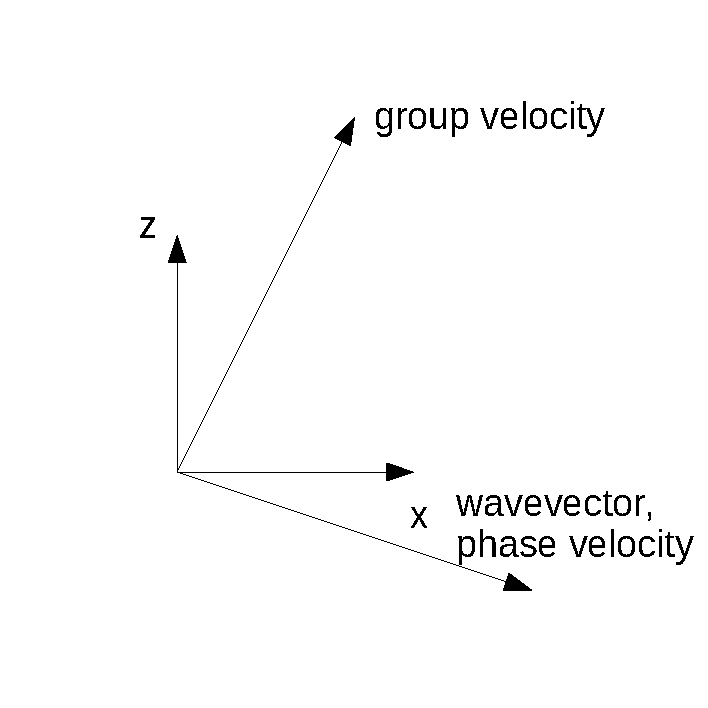
\includegraphics[width=8cm]{igw-wave-vels.pdf}
	\caption{The geometric relationship between phase velocity, group velocity and wavevector.}
	\label{fig:igw-wave-vels}
\end{center}
\end{figure}

\section{Motion of fluid particles}

For simplicity, we consider two-dimensional motion. If $\bs{u} = (u,0,w)$ and 
\begin{align}
	u&=\hat{u} \exp(i(\bs{k}\cdot\bs{x} - \omega t)) \\
	w&=\hat{w} \exp(i(\bs{k}\cdot\bs{x} - \omega t)) \\
\end{align}
then $\divg\bs{u}=0$ gives
\begin{equation}
	\hat{u} = -\frac{m}{k}\hat{w}
\end{equation}
which tells us that fluid particles oscillate parallel to the group velocity and
perpendicularly to the wavevector. We can obtain the displacements by
integrating with respect to time, or equivalently by dividing by $-i\omega$. 

\section{Equipartition of energy}

Dotting (\ref{govlinbous-mom}) with $\bs{u}$ and some manipulation gives us
\begin{equation}
	\dpd{}{t}\left(\frac{1}{2}\rho_0 \bs{u}^2 + \frac{1}{2}\frac{g^2}{\rho_0N^2}\rho'^2\right) + \divg(p'\bs{u}) = 0,
\end{equation}
the equation of conservation of energy. We identify $ \frac{1}{2}\rho_0 \bs{u}^2
$ as kinetic energy density and $\frac{1}{2}\frac{g^2}{\rho_0N^2}\rho'^2$ as
potential energy density. (Energy density is energy per unit volume, with
dimensions $\mathrm{L}^{-1} \mathrm{T}^{-2}$.) And we identify $p'\bs{u}$ as the
flux of energy per unit area.

In integral form, we can write
\begin{equation}
    \dpd{}{t} \int_V (KE + PE) \dif V + \int_S \bs{F}_E \cdot \bs{n} \dif S = 0
\end{equation}
where $KE$ is the kinetic energy density, $PE$ is the potential energy density,
and $\bs{F}_E$ is the energy flux.

%TODO
Consider a normal mode with phase $\phi' = \bs{k}'\cdot\bs{x}' - \omega t$. In a
rotated coordinate system, where $w'$ now means the velocity component along the
wave ray, we have 
\begin{align}
    w' &= \omega \eta_0 \sin\phi' \\
    b &= \frac{-\omega^2 \eta_0}{cos\theta} \cos\phi' \\
    p' &= \frac{-\rho_0 \omega^2 \eta_0 \tan\theta}{k'} \sin\phi'
\end{align}
with the other two components of velocity being zero. Thus
\begin{align}
    KE &= \frac{1}{2}\rho_0 \omega^2 \eta_0^2 \sin^2\phi' \\
    PE &= \frac{1}{2}\rho_0 \omega^2 \eta_0^2 \cos^2\phi'.
\end{align}
Calculating time averages shows that
\begin{equation}
\langle\text{kinetic energy density}\rangle = \langle\text{potential energy density}\rangle
\end{equation}
which is \textit{equipartition of energy}.

The energy flux is $\bs{F}_E = \rho_0 \omega^2 \eta_0^2 \sin^2\phi' \bs{c}_g$,
and so $\bar{\bs{F}_E} = \bar{E} \bs{c}_g$. Thus the energy flux is in the
direction of the group velocity. 

%TODO

Note that we must take real parts before multiplying together any quantities. 

\section{Oscillating cylinders}

Consider a cylinder (or any other object) suspended in a stratified medium.

At time $t=0$, it is impulsively started to oscillate at frequency $\omega<N$.
The impulsive start of the cylinder generates an entire spectrum of transient
wave modes, which generates IGWs propagating at different values of
$\theta$.\footnote{Consider the Fourier transform of the Heaviside step
function.} After some time, when the transients have decayed or moved away, we
will see a single mode of IGWs propagating at $\theta = \cos^{-1} (\omega/N)$ to
the vertical. 

If the cylinder is made to oscillate at a frequency $\omega > N$, then the waves
produced will be evanescent. The cylinder will create local disturbances which
do not travel very far.

\section{Reflections}
\subsection{Properties of reflected beams}

\begin{figure}
\begin{center}
	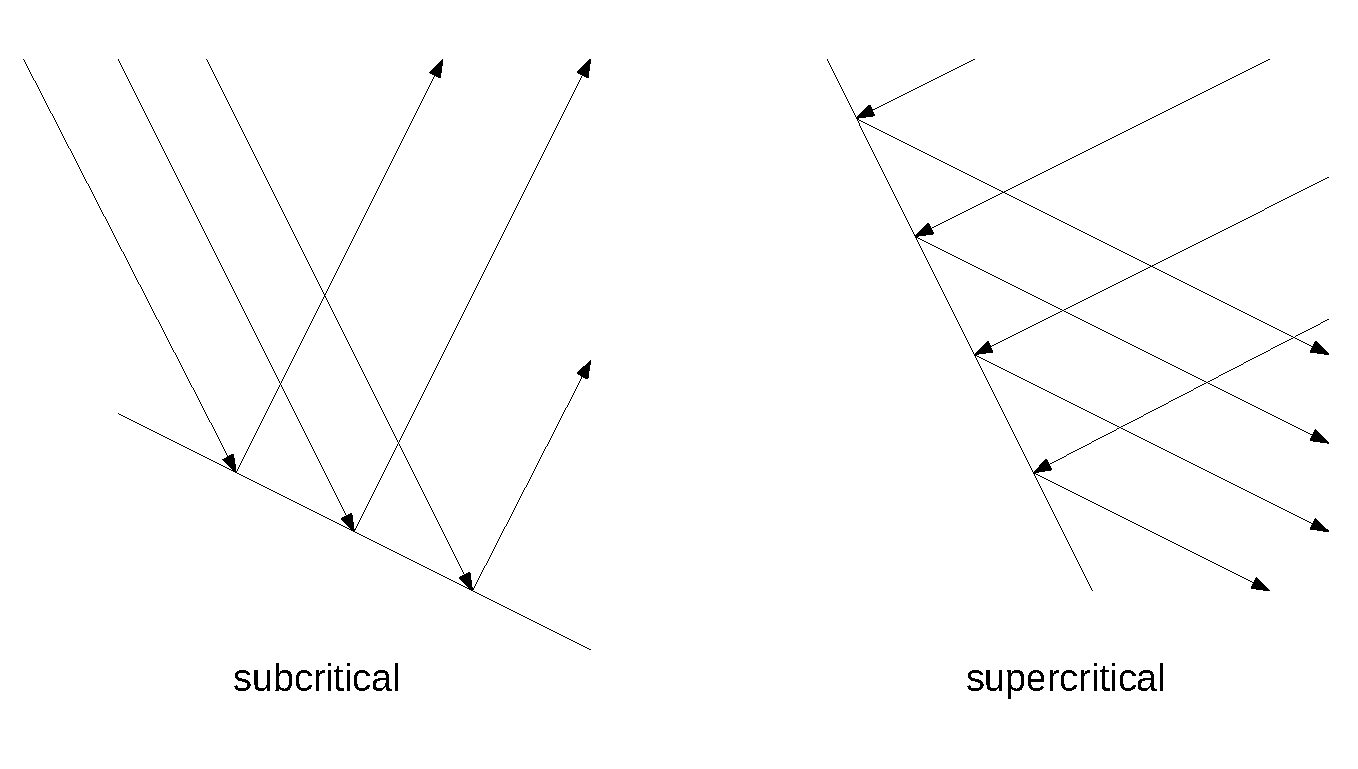
\includegraphics[width=14cm]{super-and-sub-critical.pdf}
	\caption{Super- and sub-critical reflections.}
	\label{fig:supersubcrit}
\end{center}
\end{figure}


At a boundary, the normal velocity component must be continuous. For a rigid stationary boundary, this means that the normal velocity component must vanish.

Suppose $z=0$ is a rigid stationary boundary, with a plane wave incident from $z>0$. What is the reflected wave? We have 
\begin{align}
	w &= w_I + w_R \\
	w_I &= \hat{w}_I \exp(i(\bs{k}_I\cdot\bs{x} - \omega t)) \\
	w_R &= \hat{w}_I \exp(i(\bs{k}_R\cdot\bs{x} - \omega t));
\end{align}
the two waves must have the same $\omega$ and $k_I = k_R$; the boundary condition gives $\hat{w}_I + \hat{w}_R = 0$. And causality implies that $m_R = -m_I$. 

When a plane wave reflects off a flat boundary, the incident and reflected waves
make the same angle (but reflected) with the vertical or horizontal, so that the
two waves have the same frequency $\omega = N\cos\theta$. (Note that for IGWs,
$\theta$ always represents the angle between a wave's direction and the
vertical.) In general, the angle of incidence and angle of reflection are not
equal. Depending on how the angle of the incident wave compares with the slope
of the boundary, one of two things may happen: see Figure
\ref{fig:supersubcrit}. 

From Figure \ref{fig:supersubcrit} we can see that reflections change the
wavenumber of the wave and can act to focus or defocus the rays, depending on
direction. Let $\alpha$ be the angle that the plane boundary makes with the
vertical. We define the quantity 
\begin{equation}
	\gamma  =  \frac{\sin(\alpha-\theta)}{\sin(\alpha+\theta)}
\end{equation}
to characterise the \textit{focusing power} of a reflection. 

After a lot of manipulation, we can show that focusing reflections change the amplitude and wavenumber according to
\begin{align}
	k_R  &= \gamma k_I \\
	A_R &= \gamma A_I 
\end{align}
and that defocusing reflections have the opposite effect:
\begin{align}
	k_R  &= \gamma^{-1} k_I \\
	A_R &= \gamma^{-1} A_I.
\end{align}
Thus the magnitudes of the phase velocity and group velocity change as well,
since
\begin{align}
    |\bs{c}_p| &= \frac{N}{|\bs{k}|} \cos\theta \\
    |\bs{c}_g| &= \frac{N}{|\bs{k}|} \sin\theta 
\end{align}

\subsection{Energy density upon reflection}

The energy density per unit wavelength is 
\begin{equation}
	\tilde{E} \sim \lambda A^2.
\end{equation}
After a focusing reflection, $\lambda$ is divided by $\gamma$ but $A$ is multiplied by $\gamma$, so $\tilde{E}$ is multiplied by $\gamma$. Hence the energy density per wavelength is increased after a focusing reflection. 

The energy density per unit length is 
\begin{equation}
	\hat{E} = \frac{1}{\lambda} \tilde{E}
\end{equation}
and so $\hat{E}$ is multiplied by $\gamma^2$ after a focusing reflection.

\subsection{Subcritical and supercritical reflections}

In a subcritical reflection, the boundary has a shallower slope than the wave
($\theta < \alpha$), and the vertical propagation of the wave is reversed by the
reflection. The horizontal direction of propagation is maintained.

In a supercritical reflection, $\theta > \alpha$ and the vertical direction of
propagation is maintained but the horizontal direction is reversed. 

When $\theta$ and $\alpha$ are very similar, then $\gamma$ becomes very large.
Waves will have very large amplitudes, and nonlinear effects and viscosity,
which we had ignored from the outset, become important. 

\section{Ray tracing}

Since the frequency $\omega$ is preserved upon reflection, the angle to the vertical $\theta$ is conserved. Waves therefore tend to propagate along well-defined rays. The dispersion relation alone does not tell us which way a wave propagates. We must pay attention to \textit{causality}, the fact that waves propagate away from whatever generates a disturbance. 

Our analysis so far deals with waves which are a linear perturbation from an equilibrium configuration. We have seen that when a wave reflects from a rigid surface, the reflected wave may have a larger amplitude than the incident wave. Depending on the shape of the domain and its boundaries, repeated reflections may increase the amplitude of waves and cause nonlinear effects to become important. In particular, repeated reflections can lead to trapping, to amplitudes increasing, and eventually to wave-breaking. 

\section{Wave attractors}
\subsection{Rectangular basins}
\subsection{Trapezoidal basin}
\subsection{More complex geometries}
\subsection{Energy spectrum for attractor}

\section{Decay along a beam}

So far we have completely ignored viscosity. But when a beam of waves
travels across long distances, a small viscosity may be enough to cause
significant energy losses along the beam. In this section, we reintroduce a
constant viscosity $\nu$, and consider the long-distance behaviour of beams. 

The equations of motions are
\begin{align}
	\dpd{u}{t} + \frac{1}{\rho_0}\dpd{p}{x} &= \nu\grad^2 u \\
	\dpd{w}{t} + \frac{1}{\rho_0}\dpd{p}{z} - b &= \nu\grad^2 w \\
	\dpd{b}{t} + N^2w &= 0 \\
	\divg\bs{u} &= 0
\end{align}
where 
\begin{equation}
	b = \displaystyle\frac{-g}{\rho_0} (\rho-\rho_0)
\end{equation}
is the buoyancy. 

Introduce a streamfunction $\psi$ such that $(u,w) = (-\psi_z, \psi_x)$. We have 
\begin{align}
    \dpd{b}{t} + N^2 \dpd{\psi}{x} &= 0 \\
    \dpd{}{t} \grad^2 \psi - \dpd{b}{t} - \nu \grad^4 \psi &= 0
\end{align}
Then some cross-differentiation eliminates $p$ and $b$ to give
\begin{equation}
	\grad^2 \psi_{tt} + N^2 \psi_{xx} = \nu\grad^4 \psi_t. \label{igw-damped}
\end{equation} 

The $\nu\grad^4\psi_t$ term acts to damp waves. (Along with the
$\grad^2\psi_{tt}$ term, these look like the diffusion equation for
$\grad^2\psi_t$.) We could look for plane-wave solutions to (\ref{igw-damped})
in the usual way, and obtain the dispersion relation
\begin{equation}
	\omega^2 + i\nu(k^2+m^2)\omega - N^2\cos^2\theta = 0
	\label{igwdisprel-damped}
\end{equation}
where $\cos\theta = k/|\bs{k}|$ as usual. Given $(k,m)$, we could solve
the quadratic (\ref{igwdisprel-damped}) for $\omega$. 

But often we are more interested in the spatial decay of a beam that is
generated by oscillations at a fixed $\omega$. We expect that the beam would
still propagate in the direction $\theta = \cos^{-1} (\omega/N)$, but with a
decaying amplitude. Thus we define a scaled coordinate 
$\chi = \frac{\epsilon}{\sin\theta} \xi$, where $\xi$ is the unscaled coordinate
along the beam. Let $\zeta$ be the unscaled cross-beam coordinate.

We let $\epsilon = \nu/2$ and we expand $\psi$ and $b$ as perturbation series:
\begin{align}
    \psi &= (\psi_0 + \epsilon \psi_1 + ...)\exp(i\omega t) \\
    b &= (b_0 + \epsilon b_1 + ... ) \exp(i\omega t).
\end{align}
Substituting into the governing equations and comparing orders of $\epsilon$
gives us 
\begin{equation}
    \dpd[4]{\psi_0}{\zeta} = i\dmd{\psi_0}{2}{\zeta}{}{\chi}{}
\end{equation}
and some work will give 
\begin{equation}
    \psi_0 = A \exp(ik\zeta - k^3 \chi)
\end{equation}
for some constant $A$. Thus the velocity decays exponentially along the beam;
waves with higher wavenumbers decay faster. In the environment, IGWs have
wavelengths on the order of hundreds of metres, but in the lab the wavelengths
are much smaller, on the order of a few centimetres. These have much higher
wavenumbers and decay very quickly.

We could also consider energy losses due to the diffusion of buoyancy (or
equivalently of temperature) instead of the diffusion of momentum. The relative
importance of the two diffusion processes is quantified by the Prandtl number
$\mathrm{Pr} = \nu/\kappa$. In practice, $\mathrm{Pr}$ is often $O(1)$ and both
effects may be important. For air, $\mathrm{Pr} \approx 0.7$ and for water,
$\mathrm{Pr} \approx 7$. 

\section{Reflections from rough topology}

Consider a wave beam of wavenumber $k_0$, making an angle $\theta$ with the
vertical, reflecting from a sinusoidal topography
\begin{equation}
    z = h = h_0 \sin k_T x
\end{equation}
where $k_T$ is the `wavenumber' of the topography. The incident beam is
propagating downwards and to the right. We suppose that the height of the
topography, $h_0$, is small (more precisely, that $h_0 k_T \ll 1$).

Suppose the incident beam would reach $z = 0$ at $x = x_0$, were it not for the
topography. The equation of the beam is therefore given by
\begin{equation}
    z = \beta (x_0 - x)
\end{equation}
where $\beta = 1/\tan \theta$. The beam intersects the topography at the point
$x = x_i$, where $x_i$ solves
\begin{equation}
    h_0 \sin k_T x_i = \beta (x_0 - x_i).
\end{equation}
Define $\delta x = x_i - x_0$

\subsection{Subcritical reflection from a sinusoidal}

If the slope of the topography is sufficiently small, then all ray reflections
will be subcritical and ray tracing suggests that an incident wavebeam should be
reflected forwards. 

If $k_0 < k_T$, so the wavelength of the incident beam is larger than the
wavelength of the topography, then we get \textit{back scatter}: The reflected
wave propagates upwards but to the \textit{left}. This is because the group
velocity of the reflected wave must be upwards.

\subsection{Supercritical reflections from a sinusoidal}

\paragraph{Steep topography} If instead we had steep topography, with $h_0 k_T
\gg 1$, then the picture is much more complicated. Rays can bounce multiple
times off the topography before leaving. We will observe both forward scatter
and back scatter. The amounts of energy that scatter forwards and backwards
depends very sensitively on the incident angle $\theta$, and it is not possible
to write down a formula for these amounts (although it is possible to bound
them).

Moreover, attractors may form in the deep gaps between the topography. These may
cause the amplitude of the wave to increase so much that wave breaking starts to
occur. The inviscid approximation also becomes invalid, because steep velocity
gradients will form. Mixing may occur, destroying the original stratification. 

\section{Non-linear stratification}

If $N$ is not constant but varies with $z$ (say), then waves will not follow
straight paths but will refract, and may also reflect.

\subsection{Very sharp changes}

Consider a stratification with $N = N_1$ in $z < 0$ and $N = N_2$ in $z > 0$,
where $N_2 < N_1$. Consider a wave incident from $z < 0$ with frequency
$\omega$. The incident wave's angle to the vertical $\theta_i$ is given by $\cos
\theta_i = \omega/N_1$.  A transmitted wave in $z > 0$ will make an angle
$\theta_t$ to the vertical, where $\cos\theta_t = \omega/N_2$. In order that the
boundary conditions be satisfied, there will also need to be a
\textit{reflected} wave propagating downwards from $z = 0$. Thus we have
\textit{total internal reflection}. 

Note that if $N_2 < \omega < N_1$ then the transmitted wave will be evanescent.

\subsection{Very slow changes}

If $N$ varies very slowly with $z$, over
lengthscales much larger than a wavelength, then the WKB method can be used to
find the trajectory of a wave. 

The frequency $\omega$ of a wave is still constant, and we assume that $\omega$
is still related to $\theta$, the angle between the direction of propagation and
the vertical, by
\begin{equation}
 \omega = N(z)\cos\theta.
\end{equation}
Since $\omega$ is fixed, this determines $\theta = \theta(z)$, which allows us
to solve for the path of the ray. Say the ray is given by $x = X(z)$. Then
\begin{equation}
    \dod{X}{z} = \tan \theta = \frac{\sqrt{1 - \cos^2 \theta}}{\cos\theta}.
\end{equation}

For example, consider $N(z) = N_0 e^{-z/H}$, so that $\cos\theta(z) =
(\omega/N_0) e^{z/H}$. Then we have 
\begin{equation}
    \dod{X}{z} = \sqrt{1 - \cos^2 \theta_0 e^{2z/H}} \frac{e^{-z/H}}{\cos\theta_0}.
\end{equation}

As $z$ increases, $N$ decreases. Eventually we will have $\omega/N \rightarrow
1$, $\od{X}{z} \rightarrow \infty$ and the wave can no longer propagate upwards.
Instead, the wave is reflected back downwards. (In practice, the amplitude of
the wave also grows as we approach $\omega/N\rightarrow1$, so that nonlinear
processes start to play a role as well.)

\section{Leewaves}

When a medium flows past an obstacle, a wake may form. It may be possible to
have standing (stationary) waves in the wake, with a particular wavenumber and
frequency.  When standing internal gravity waves occur in the atmosphere as a
wind flows past obstacles such as mountains, these are known as
\textit{leewaves}.

\subsection{Kelvin ship waves}

As an aside to introduce standing waves, we consider a ship moving with velocity
$\bs{U} = U\bs{e}_x$ in deep water. The surface waves in deep water have a
dispersion relation
\begin{equation}
\omega^2 = g|\bs{k}|
\end{equation}
and phase
\begin{equation}
	\phi = \bs{k}\cdot\bs{x} - \omega t.
\end{equation}
Let $\bs{x}'$ denote a position vector relative to the ship, so that $\bs{x}' =
\bs{x} - \bs{U}t$. Then
\begin{equation}
	\phi = \bs{k}\cdot\bs{x}' + (\bs{k}\cdot\bs{U} - \omega) t.
\end{equation}
Hence waves that are stationary in the frame of the ship have
\begin{align}
	\bs{k}\cdot\bs{U} &= \omega \\
	U\cos\theta &= |\bs{c}_g|
\end{align}
where, in this section, $\theta$ is the angle between $\bs{U}$ and $\bs{k}$. 

For these waves, $\bs{c}_g$ and $\bs{c}_p$ are parallel, and $|\bs{c}_g| =
\frac{1}{2} |\bs{c}_p| = \frac{1}{2}U\cos\theta$. This is the speed at which
wave packets travel. Some geometry then tells us the shape that these waves make
behind the ship.

In shallow water, surface waves are not dispersive and such stationary waves are
not seen.

\subsection{Extended range of hills}

Now we return to considering internal gravity waves. We consider leewaves, which
are stationary atmospheric IGW. A wind of speed $U$ flows, from left to right,
over a sinusoidal mountain range with wavelength $\lambda_T$ and so
topographical wavenumber $k_T = 2\pi/\lambda$. 

Because the leewaves are stationary in the frame of the mountains, an observer
in this frame sees the phase of the wave as unchanging in time. The frequency of
the forcing must therefore be
\begin{equation}
	\omega = k_T U = \frac{2\pi U}{\lambda_T}
\end{equation}
and the wave crests make an angle $\theta = \cos^{-1} (\omega/N)$ with the
vertical. The phase velocity is aligned with the wave crests, so that the
observer sees the waves as being stationary.

We move to a frame moving with the wind, in which the mountains are moving with
speed $U$ to the left. This does not change the angle between the wave crests
and the vertical, but the group velocity in this frame is $\bs{c}'_g = \bs{c}_g
- \bs{U}$, which (by geometry) is \textit{aligned with the crests}. 

\subsection{Flow over a bump}

Now instead of a sinusoidal range of hills we consider a single hill in
otherwise flat terrain. This corresponds to a whole spectrum of Fourier
components, as we see by considering the Fourier transform of a localised bump
(such as $\exp(-x^2/L^2)$. This hill will therefore excite a whole spectrum of
waves.

\paragraph{Principle of stationary phase} Consider the phase
\begin{equation}
    \phi = \bs{k}\cdot\bs{x} - \omega t.
\end{equation}
Differentiating, we have
\begin{equation}
    \dif\phi = \dpd{\phi}{k_i} \dif k_i + \dpd{\phi}{x_i} \dif x_i +
    \dpd{\phi}{\omega} \dif \omega + \dpd{\phi}{t} \dif t 
      = \dpd{\phi}{x_i} \dif x_i + \dpd{\phi}{t} \dif t
\end{equation}
assuming that $\dif\bs{k}$ and $\dif\omega$ both vanish. The \textit{principle
of stationary phase} says that an observer will see leewaves with $\dif\phi=0$.

For an observer moving at $(V,0,0)$, with constant $V$, the condition
$\dif\phi=0$ therefore becomes
\begin{equation}
    V\dpd{\phi}{x} + \dpd{\phi}{t} = 0
\end{equation}
and so
\begin{equation}
    V k_x - \omega = V|\bs{k}|\cos\theta - \omega = 0
\end{equation}
with $k_x = |\bs{k}|\cos\theta$ where $\theta$ is the angle that the crests
make to the vertical. Moreover, $\omega/N = \cos\theta$.

\subsection{Causality}

\section{Shear flows}

\subsection{Sheared base state}

Suppose the background stratified fluid is not stationary but has velocity
$\bs{U} = (U(z),0,0)$. Linearising the full governing equations of motion about
this base state by writing $\bs{u} = \bs{U} + (u',v',w')$, and a lot of
manipulation to eliminate everything apart from $w'$, eventually gives
\begin{equation}
	\left(\dpd{}{t} + U\dpd{}{x}\right)^2 \grad^2 w' + N^2 \dpd[2]{w'}{x} - U''\left(\dpd{}{t} + U\dpd{}{x}\right)\dpd{w'}{x} = 0.
\end{equation}
Note that this reduces to \ref{igw-govlin-w} if $U\equiv0$. If $U$ is constant, then a change of frame would recover \ref{igw-govlin-w} as expected.

For flows which are steady (in this frame of reference), we have
\begin{equation}
	\dpd[2]{}{x} \grad^2 w' + \left( \frac{N^2}{U^2} - \frac{U''}{U} \right)\dpd[2]{w'}{x} = 0.
\end{equation}
Integrating twice with respect to $x$ then gives
\begin{equation}
	\grad^2 w' + \left( \frac{N^2}{U^2} - \frac{U''}{U} \right) w' = 0.
\end{equation}

If $U$ and $N$ are constant, or very slowly varying, then we can search for plane wave solutions
\begin{equation}
	w' = w_0 e^{i(kx+mz)}
\end{equation}
which satisfy
\begin{equation}
	-(k^2 + m^2) + \frac{N^2}{U^2} = 0
\end{equation}
or $|\bs{k}| = N/U$ as before. Clearly, a similar argument shows that if
$\frac{N^2}{U^2} - \frac{U''}{U} $ is constant, then
$|\bs{k}|^2=\frac{N^2}{U^2}-\frac{U''}{U}$.

\subsection{Ray tracing in a shear flow}

When the length scale over which $U$ and $N$ change is much larger than the
wavelength of internal waves, we can consider the important wave properties as
being instantaneous in the local state of the background flow. This is the WKB
approximation. Rays follow the group velocity relative to the fluid. However, in
our frame of reference the waves appear stationary, and so the phase velocity
must be parallel to the wave crests and the group velocity antiparallel with the
wavenumber vector. We can thus take the trajectory of a wave propagating with
the mean flow as
\begin{equation}
	\dod{z}{x} = \frac{c_{gz}}{U - c_{gx}} = \frac{m}{k}
\end{equation}
where $\bs{c}_g$ is the group velocity relative to the fluid.

Recalling that $k^2 + m^2 = N^2 / U^2$, arguing that $k$ is conserved along
the ray (see below) and assuming that $U''/U \ll N^2 /U^2$, then
\begin{equation}
	m^2 = \frac{N^2}{U^2} - k^2
\end{equation}
and so 
\begin{equation}
	\dod{z}{x} = \left[\left(\frac{N}{kU}\right)^2 - 1\right]^{1/2}.
\end{equation}
Waves cannot propagate through a level where $kU/N = 1$.

The horizontal wavenumber $k$ is conserved, because the background flow $\bs{U}$
is a parallel horizontal shear flow with no dependence on $x$, and will not
`stretch' or `compress' waves in this direction. (This is similar to Noether's
theorem, with $k$ playing the role of the conjugate momentum to $x$.)

Different observers moving with the fluid will not agree on the frequency of the
wave, because $\od{z}{x}$ varies with $z$. This is equivalent to the Doppler
effect. 

In the atmosphere, $U/N$ tends to increase with height as $U$ increases.

\subsection{*Three-dimensional forcing}

\subsection{*Effect of viscosity}

We have seen already that viscosity causes dissipation which is proportional to
$|\bs{k}|^3$. 

\subsection{*Blocking}

\section{Columnar modes}
\section{*Stokes drift in internal waves}
\section{Resonant triads}
